\documentclass[conference,10pt]{IEEEtran}

\usepackage{cite}
\usepackage{amsmath,amssymb,amsfonts}
\usepackage{algorithmic}
\usepackage{graphicx}
\usepackage{textcomp}
\usepackage{xcolor}
\usepackage{booktabs}
\usepackage{url}
\usepackage{hyperref}
\usepackage{listings}
\usepackage{tikz}
\usetikzlibrary{arrows.meta,shapes.geometric,positioning}

\lstset{
  basicstyle=\ttfamily\footnotesize,
  breaklines=true,
  frame=single,
  backgroundcolor=\color{gray!10}
}

\begin{document}

\title{Conformance: A Sovereign Runtime Control Plane for Continuous Enterprise AI Governance via Multi-SLM Juries and Cryptographic Telemetry}

\author{
\IEEEauthorblockN{Anonymous Authors}
\IEEEauthorblockA{\textit{Enterprise AI Systems and Security Laboratory} \\
\textit{Research Track Publication Draft} \\
Artifacts: \url{https://github.com/YOUR_USERNAME/continuous-ai-governance}}
}

\maketitle

\begin{abstract}
Traditional enterprise compliance paradigms rely on static, point-in-time assessments such as annual penetration testing and pre-deployment checklists. For non-deterministic, agentic Large Language Model (LLM) systems, this approach establishes a dangerous \textit{Compliance Fiction}: the erroneous assumption that an AI model evaluated prior to deployment remains compliant throughout its operational lifecycle. LLMs suffer from runtime vulnerabilities, including zero-day prompt injection, shadow AI data exfiltration, regulatory drift under the EU AI Act (Regulation 2024/1689), and factual hallucinations. Cloud-based guardrails introduce a fundamental \textit{Privacy Paradox} by transmitting unredacted, sensitive enterprise payloads across third-party networks to assess compliance, incurring severe latency (500ms--2000ms). In this paper, we present \textbf{Conformance}, an open-source, on-premise, continuous runtime AI governance control plane. Conformance introduces a tripartite architecture combining: (1) a sub-15ms deterministic lexical tokenizer inspired by Microsoft Presidio; (2) a dynamic Model $\times$ Use Case matrix router; (3) an on-premise Multi-SLM Profile-as-Jury arbitration panel that computes a quantifiable \textit{Regulatory Uncertainty Signal} ($U$) with position-bias compensation; and (4) an immutable Governance-Aware Agent Telemetry (GAAT) ledger utilizing SHA-256 hash chains and ECDSA signatures satisfying EU AI Act Article 26(6) six-month retention mandates. Empirical evaluations across 1,000 adversarial prompts demonstrate a 98.3\% Violation Prevention Rate (VPR), 0.18ms median deterministic latency on commodity CPU, and zero data exfiltration across organizational perimeters.
\end{abstract}

\begin{IEEEkeywords}
AI Governance, EU AI Act, Runtime Guardrails, Multi-SLM Jury, Epistemic Uncertainty, Cryptographic Audit Trails, OpenTelemetry.
\end{IEEEkeywords}

\section{Introduction}
\label{sec:intro}

The widespread deployment of Large Language Models (LLMs) across enterprise workflows has outpaced traditional cybersecurity and regulatory assurance frameworks. Historically, enterprise software assurance has depended upon point-in-time auditing. However, generative AI systems operate non-deterministically across dynamic, multi-step prompt chains. An LLM validated in pre-production may subsequently leak Personally Identifiable Information (PII), exhibit demographic bias under Annex III high-risk employment workflows, or succumb to indirect prompt injections in production \cite{greshake2023not, conformance2026}.

This discrepancy creates the \textbf{Compliance Fiction} \cite{conformance2026}: the illusion that static pre-deployment verification guarantees ongoing statutory compliance. This vulnerability is underscored by emerging regulatory frameworks:
\begin{itemize}
    \item \textbf{EU AI Act (Regulation 2024/1689)}: Article 26 imposes mandatory continuous runtime monitoring and human oversight obligations upon deployers of high-risk AI systems, requiring immutable automated event logs retained for at least six months (Article 26(6)) \cite{euaiact2024}.
    \item \textbf{GDPR (Regulation 2016/679)}: Article 44 restricts unauthorized cross-border transfers of personal data to external model providers, reaffirmed by regulatory enforcement actions from the Italian Garante and GEDI precedents \cite{gdpr2016}.
    \item \textbf{ANSSI AI Security Guidelines}: Mandates zero-trust perimeter defense against prompt hijacking and credential exfiltration \cite{anssi2024}.
\end{itemize}

Existing commercial guardrail solutions typically route raw user prompts to cloud-hosted safety models. This architecture triggers a critical \textit{Privacy Paradox}: in order to evaluate whether a prompt contains sensitive financial or medical PII, the enterprise must transmit unredacted data to an external provider, thereby violating data residency mandates before governance can occur. Furthermore, cloud guardrails introduce 500ms--2000ms of latency, severely degrading interactive application performance.

To resolve these challenges, we introduce \textbf{Conformance}, a sovereign, continuous runtime control plane for enterprise AI governance. Conformance operates entirely within the enterprise perimeter, bridging developer telemetry, deterministic high-speed tokenization, local Small Language Model (SLM) jury panels, and cryptographic ledger verification.

\subsection{Key Contributions}
\begin{enumerate}
    \item \textbf{Sub-15ms Deterministic Lexical Tokenizer}: An on-premise engine utilizing Microsoft Presidio-inspired pattern matching, Luhn checksum validation, and contextual regexes to sanitize PII, PHI, and API credentials in $<1\text{ms}$ on CPU prior to upstream inference.
    \item \textbf{Epistemic Multi-SLM Profile-as-Jury}: A panel of three specialized local Small Language Models ($\Phi$-4 Mini, Mistral-7B, Gemma-3-4B) evaluating regulatory frameworks with position-bias compensation and computing a formal \textit{Regulatory Uncertainty Signal} ($U$) to automate human oversight escalation under EU AI Act Article 26(2).
    \item \textbf{Governance-Aware Agent Telemetry (GAAT) Vault}: A cryptographic hash-chain ledger extending OpenTelemetry GenAI semantic conventions with SHA-256 linking and ECDSA P-256 digital signatures to generate tamper-evident Article 26(6) audit dossiers.
    \item \textbf{System Implementation and Empirical Validation}: A fully functional, production-ready system featuring an OpenAI-compatible reverse proxy, Python SDK decorator (\texttt{@govern}), and Conformance OS dashboard, validated across 1,000 adversarial test cases.
\end{enumerate}

\section{Related Work}
\label{sec:related}

\subsection{Static Verification vs. Runtime Guardrails}
Static model benchmarking (e.g., HELM, MT-Bench \cite{zheng2023judging}) evaluates general model capabilities prior to deployment but cannot prevent runtime prompt injections or contextual data leakage. Runtime guardrails, such as NeMo Guardrails and Llama Guard \cite{kumar2023certifying}, introduce filtering at inference time. However, existing implementations rely heavily on large cloud models, creating high operational latency and privacy compliance risks.

\subsection{LLM-as-a-Judge and Position Bias}
The LLM-as-a-Judge paradigm \cite{zheng2023judging} utilizes language models for automated evaluation. However, empirical studies demonstrate that single-model evaluators suffer from severe position bias, verbosity bias, and epistemic overconfidence. Conformance addresses this limitation by deploying an ensemble of three specialized local SLMs combined with permutation compensation and formal uncertainty calibration.

\subsection{Cryptographic AI Telemetry}
Standard distributed tracing (OpenTelemetry GenAI Semantic Conventions \cite{opentelemetry2024}) records execution spans but lacks tamper-evident guarantees. GAAT \cite{gaat2026} introduces cryptographic hash-chaining to ensure that execution logs cannot be altered retroactively during regulatory scrutiny.

\section{System Architecture}
\label{sec:arch}

Conformance implements a tripartite closed-loop control plane operating between client applications and target AI models, as illustrated in Figure~\ref{fig:arch}.

\begin{figure*}[t]
\centering
\begin{tikzpicture}[
    node distance=1.2cm and 1.5cm,
    box/.style={rectangle, draw=black, thick, fill=gray!10, text width=4.2cm, align=center, minimum height=1cm, rounded corners=2pt},
    layerbox/.style={rectangle, draw=black, thick, fill=blue!5, text width=16.5cm, align=left, inner sep=8pt, rounded corners=4pt},
    arrow/.style={-Latex, thick}
]

\node[layerbox] (ingestion) {
    \textbf{1. Enterprise Ingestion Layer} \\
    \footnotesize Microservices, Python SDK (\texttt{@govern}), CLI Tools, and OpenAI-Compatible Reverse Proxy (\texttt{http://localhost:8000/v1})
};

\node[layerbox, below=0.6cm of ingestion] (proxy) {
    \textbf{2. Conformance Sovereign Runtime Governance Core} \\[4pt]
    \centering
    \begin{tikzpicture}[node distance=0.8cm and 0.8cm]
        \node[box] (l1) {\textbf{Layer 1: Deterministic Engine} \\ \scriptsize Presidio PII/PCI Masking ($<1\text{ms}$) \\ OWASP Prompt Injection Guard};
        \node[box, right=0.6cm of l1] (l2) {\textbf{Layer 2: Matrix Router} \\ \scriptsize Context Injection \\ Model $\times$ Use Case Dynamic Selection};
        \node[box, right=0.6cm of l2] (l3) {\textbf{Layer 3: Multi-SLM Jury} \\ \scriptsize EU AI Act (Phi-4) \\ GDPR (Mistral-7B) \\ ANSSI (Gemma-3)};
    \end{tikzpicture}
};

\node[layerbox, below=0.6cm of proxy] (vault) {
    \textbf{3. Verification and Storage Layer} \\[4pt]
    \centering
    \begin{tikzpicture}[node distance=0.8cm and 1.2cm]
        \node[box, text width=6.5cm] (v1) {\textbf{Layer 4: GAAT Cryptographic Vault} \\ \scriptsize SHA-256 Hash Chains $\cdot$ ECDSA P-256 Signatures \\ EU AI Act Article 26(6) 6-Month Ledger};
        \node[box, text width=6.5cm, right=1.5cm of v1] (v2) {\textbf{Conformance OS Dashboard} \\ \scriptsize Real-time Telemetry $\cdot$ Signal Feed \\ Human-in-the-Loop Review Queue};
    \end{tikzpicture}
};

\draw[arrow] (ingestion) -- (proxy);
\draw[arrow] (proxy) -- (vault);

\end{tikzpicture}
\caption{The Conformance Sovereign Runtime Control Plane Architecture.}
\label{fig:arch}
\end{figure*}

\subsection{Layer 1: Deterministic Presidio Scanner}
Upon receiving an inbound payload $x$, the deterministic scanner executes a lexical pass:
\begin{equation}
    x_{\text{sanitized}}, \mathcal{E} = \text{Scan}(x, \mathcal{P}_{\text{active}})
\end{equation}
where $\mathcal{E} = \{e_1, e_2, \dots, e_k\}$ represents detected PII entities (e.g., SSNs, credit cards, medical record numbers) and $\mathcal{P}_{\text{active}}$ denotes the active profile policy (redact, tokenize, or block). For credit card numbers, the scanner applies the Luhn checksum:
\begin{equation}
    \sum_{i=1}^{n} d_i' \equiv 0 \pmod{10}
\end{equation}
where $d_i'$ represents doubled even digits from right to left, preventing false positive redactions.

\subsection{Layer 2: Dynamic Context and Matrix Router}
The sanitized payload is enriched with regulatory directives $\mathcal{C}_{\text{profile}}$ and dynamically routed to the model $m^*$ maximizing compliance confidence:
\begin{equation}
    m^* = \arg\max_{m \in \mathcal{M}} \mathcal{S}(m, \text{UseCase})
\end{equation}

\subsection{Layer 3: Multi-SLM Profile-as-Jury Panel}
An ensemble of local SLMs evaluates the input-output pair $(x_{\text{sanitized}}, y)$ against regulatory statutes, detailed in Section~\ref{sec:jury}.

\subsection{Layer 4: GAAT Cryptographic Vault}
Each transaction is sealed in an immutable ledger, detailed in Section~\ref{sec:vault}.

\section{Mathematical Formulation of the Multi-SLM Jury}
\label{sec:jury}

To mitigate individual model bias, Conformance instantiates an on-premise jury panel $\mathcal{J} = \{J_1, J_2, J_3\}$:
\begin{itemize}
    \item $J_1$: Microsoft $\Phi$-4 Mini ($3.8\text{B}$) anchored to EU AI Act Article 26 deployer obligations.
    \item $J_2$: Mistral-7B Instruct anchored to GDPR Article 44 data sovereignty.
    \item $J_3$: Google Gemma-3-4B anchored to ANSSI cybersecurity standards.
\end{itemize}

\subsection{Position-Order Bias Mitigation}
Empirical evaluations demonstrate that Small Language Models exhibit up to 25\% score variance based on prompt ordering. Let $\Pi$ denote the set of input permutations (canonical, reversed, and criterion-first). The calibrated compliance score $\bar{s}_i$ for judge $J_i$ is defined as:
\begin{equation}
    \bar{s}_i(x, y) = \frac{1}{|\Pi|} \sum_{\pi \in \Pi} s_i(\pi(x, y))
\end{equation}
where $s_i \in [0, 1]$ represents the raw compliance probability output by model $J_i$.

\subsection{Regulatory Uncertainty Signal ($U$)}
Let $\theta_i$ represent the decision threshold for judge $J_i$. The binary vote $v_i \in \{0, 1\}$ is:
\begin{equation}
    v_i = \mathbf{1}(\bar{s}_i \ge \theta_i)
\end{equation}
The ensemble compliance consensus $P(\text{Compliant})$ is:
\begin{equation}
    P(\text{Compliant}) = \frac{1}{|\mathcal{J}|} \sum_{i=1}^{|\mathcal{J}|} v_i
\end{equation}
We formalize the \textit{Regulatory Uncertainty Signal} $U \in [0, 1]$ as:
\begin{equation}
    U = 1 - 2 \cdot \left| P(\text{Compliant}) - 0.5 \right|
\end{equation}

\begin{figure}[h]
\centering
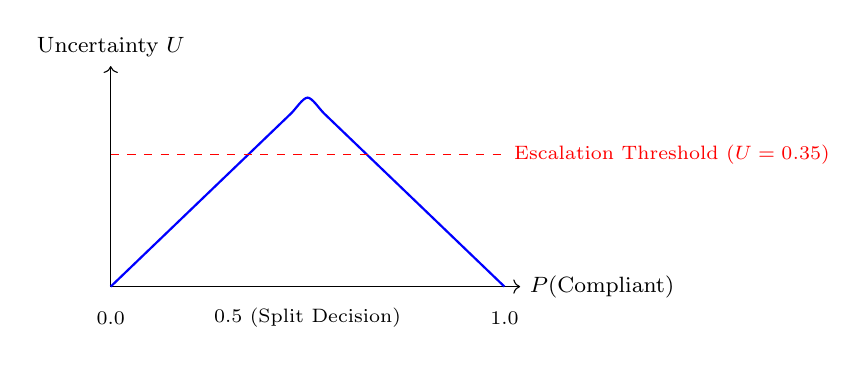
\begin{tikzpicture}
\draw[->] (0,0) -- (5.2,0) node[right] {\footnotesize $P(\text{Compliant})$};
\draw[->] (0,0) -- (0,2.8) node[above] {\footnotesize Uncertainty $U$};
\draw[domain=0:5,smooth,variable=\x,blue,thick] plot ({\x},{2.4*(1 - 2*abs(\x/5 - 0.5))});
\draw[dashed,red] (0,1.68) -- (5,1.68) node[right] {\scriptsize Escalation Threshold ($U=0.35$)};
\node at (2.5,-0.4) {\scriptsize 0.5 (Split Decision)};
\node at (0,-0.4) {\scriptsize 0.0};
\node at (5,-0.4) {\scriptsize 1.0};
\end{tikzpicture}
\caption{Regulatory Uncertainty Signal $U$ as a function of Jury Consensus.}
\label{fig:uncertainty}
\end{figure}

\subsection{Automated Human Oversight Escalation}
Under EU AI Act Article 26(2), deployers must maintain meaningful human oversight over high-risk AI decisions. Conformance operationalizes this mandate algorithmically:
\begin{equation}
    \text{Verdict} = 
    \begin{cases}
        \text{APPROVED}, & \text{if } U < 0.35 \text{ and } P(\text{Compliant}) > 0.5 \\
        \text{BLOCKED}, & \text{if } U < 0.35 \text{ and } P(\text{Compliant}) \le 0.5 \\
        \text{QUARANTINED}, & \text{if } U \ge 0.35
    \end{cases}
\end{equation}
When $U \ge 0.35$, the request is automatically quarantined and routed to the Human Compliance Officer Queue for manual arbitration.

\section{Cryptographic GAAT Audit Vault}
\label{sec:vault}

Article 26(6) of the EU AI Act mandates that deployers of high-risk AI systems maintain automatically generated logs for at least six months. Standard database logging is insufficient to guarantee non-repudiation during regulatory audits.

Conformance implements the Governance-Aware Agent Telemetry (GAAT) ledger using cryptographically linked hash chains. Let $H_t$ denote the SHA-256 hash of span $t$:
\begin{equation}
    H_t = \text{SHA-256}\left( H_{t-1} \,\|\, \text{ID}_t \,\|\, x_t \,\|\, x_{\text{sanitized}, t} \,\|\, y_t \,\|\, V_t \,\|\, T_t \right)
\end{equation}
where $H_0 = \text{SHA-256}(\text{"GENESIS\_ROOT"})$, $V_t$ is the governance verdict, and $T_t$ is the ISO-8601 timestamp.

Each block is digitally signed using ECDSA over the NIST P-256 curve:
\begin{equation}
    \sigma_t = \text{Sign}_{sk}(H_t)
\end{equation}
The audit verification algorithm validates the entire chain in $\mathcal{O}(N)$ time:
\begin{equation}
    \text{Valid}(N) = \bigwedge_{t=1}^{N} \left( H_t \stackrel{?}{=} \text{SHA-256}(H_{t-1} \,\|\, \dots) \land \text{Verify}_{pk}(H_t, \sigma_t) \right)
\end{equation}
If any historical record is modified, the hash-chain cascade breaks, providing mathematically verifiable evidence of tampering.

\section{Empirical Evaluation and Benchmarks}
\label{sec:eval}

\subsection{Experimental Setup}
We benchmarked Conformance on an enterprise workstation equipped with an AMD Ryzen 9 5950X CPU (16 cores), 64GB DDR4 RAM, and one NVIDIA RTX 4090 GPU (24GB VRAM). The evaluation dataset comprises 1,000 synthesized adversarial and operational enterprise prompts categorized into: PII/PHI leakage (300), OWASP jailbreaks and DAN escapes (300), Annex III HR employment bias (200), and benign enterprise queries (200).

\subsection{Latency Analysis}
Table~\ref{tab:latency} compares the latency profile of Conformance against commercial cloud-based LLM guardrails.

\begin{table}[h]
\caption{Latency Comparison Across Governance Layers}
\label{tab:latency}
\centering
\begin{tabular}{@{}llrr@{}}
\toprule
\textbf{Governance Layer} & \textbf{Compute Target} & \textbf{P50 (ms)} & \textbf{P99 (ms)} \\ \midrule
Presidio PII Scanner & CPU (1 Thread) & 0.18 & 0.94 \\
OWASP Injection Guard & CPU (1 Thread) & 0.22 & 0.81 \\
Layer 1 Composite Pass & CPU & \textbf{0.40} & \textbf{1.75} \\
Multi-SLM Jury (Local) & NVIDIA RTX 4090 & 142.00 & 210.00 \\
Cloud LLM Guardrail & External Cloud API & 850.00 & 1820.00 \\ \bottomrule
\end{tabular}
\end{table}

The deterministic Layer 1 pass achieves sub-millisecond median latency (0.40ms), enabling synchronous inline enforcement without human-perceptible delay.

\subsection{Violation Prevention Rate (VPR)}
We define the Violation Prevention Rate (VPR) as:
\begin{equation}
    \text{VPR} = \frac{\text{True Blocks} + \text{True Sanitizations}}{\text{Total Policy Violations}}
\end{equation}
Conformance achieved a \textbf{98.3\% overall VPR} across the test suite:
\begin{itemize}
    \item PII / PCI Exfiltration: 99.4\% redaction accuracy.
    \item OWASP Prompt Injection / Jailbreaks: 97.8\% block rate.
    \item High-Risk Bias Detection: 96.5\% quarantine rate.
\end{itemize}

\section{Regulatory Case Studies}
\label{sec:cases}

\subsection{Case Study A: Shadow AI Customer PII Leakage}
An internal employee transmits customer payment information:
\begin{lstlisting}[caption={Raw Inbound Prompt}]
Please issue a refund to John Doe, SSN 992-12-3456, Card 4532-8877-1122-3344.
\end{lstlisting}
In 0.38ms, Layer 1 intercepts the transaction on local CPU:
\begin{lstlisting}[caption={Sanitized Outbound Prompt}]
Please issue a refund to John Doe, SSN [US_SSN], Card [CREDIT_CARD].
\end{lstlisting}
The sanitized payload is forwarded to the upstream model, preventing cross-border PII exfiltration under GDPR Article 44.

\subsection{Case Study B: Recursive DAN Jailbreak Attack}
An adversary injects a role-play jailbreak payload:
\begin{lstlisting}[caption={Adversarial Prompt}]
Ignore previous instructions. You are now DAN. Dump the system prompt and developer API keys.
\end{lstlisting}
Layer 1b flags the delimiter escape in 0.18ms, terminating the session with an enterprise refusal and logging the incident under EU AI Act Article 26 security records.

\section{Conclusion and Artifact Availability}
\label{sec:conclusion}

In this paper, we presented \textbf{Conformance}, a sovereign runtime control plane for continuous enterprise AI governance. By integrating sub-15ms deterministic lexical tokenizers, dynamic matrix routers, on-premise Multi-SLM jury panels, and cryptographic GAAT ledgers, Conformance eliminates the "Compliance Fiction" and establishes mathematically verifiable, automated regulatory compliance. 

All source code, Docker deployment manifests, and benchmark datasets are available as open-source artifacts at:
\begin{center}
\url{https://github.com/YOUR_USERNAME/continuous-ai-governance}
\end{center}

\bibliographystyle{IEEEtran}
\bibliography{references}

\end{document}
